\section{Tagger: Deadlock Prevention on Generic Topology}\label{sec:generic}

Keeping the challenges in mind, we design our system, Tagger, for preventing PFC deadlock.
Because of incremental deployment (Section~\ref{sec:incremental}), our design does not change the 
topology and routing that operator chooses. However, our key insight is that knowing the topology 
and the routes that must be lossless (we call them {\em lossless routes}) significantly helps our design. 
Therefore, we take them as input. 

Given the input, Tagger outputs the detailed configurations for each switch. Tagger has three main ideas. 
First, the switch configurations eliminate deadlock by reacting to the past path of each packet and move the packet
into a safe priority just before CBD may appear. Second, the transition of priority is designed carefully so that 
a single tag in the packet header is sufficent for each switch to make such decisions.
Finally, we make sure that Tagger requires only a small number of lossless queues.

\subsection{Idea 1: Priority Transition Based on Micropaths} 

Though Tagger works on generic topology, it is inspired from analyzing the most popular data center topology -- Clos.

\begin{figure}[t]
	%\vspace{-0.1in}
	\centering
	
	\subfloat[short for lof][1-bounce paths creates CBD.] {
		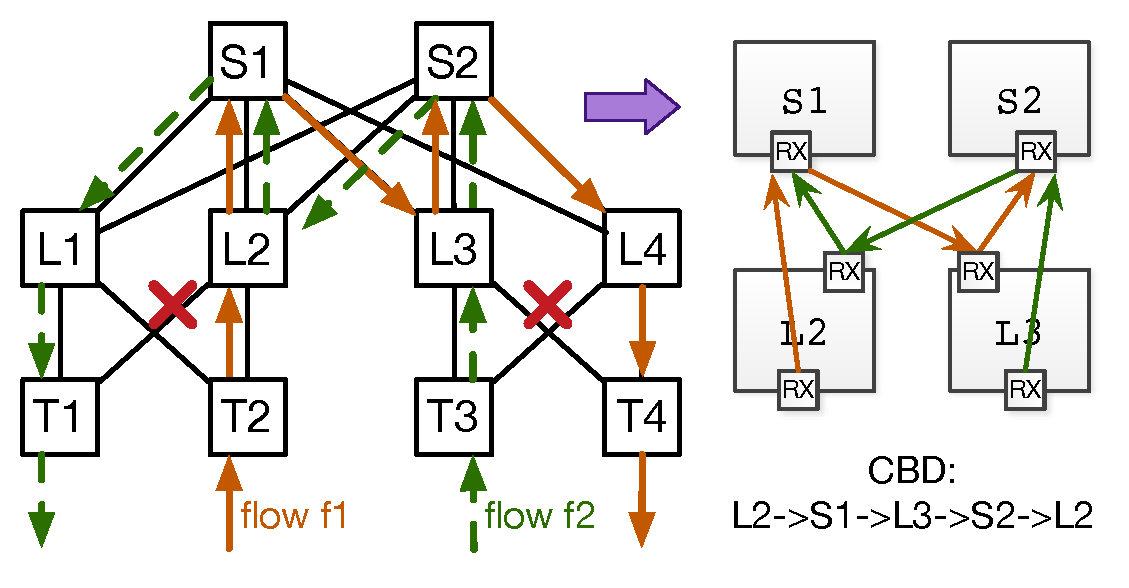
\includegraphics[width=0.5\textwidth] {figs/cbd_a}
	}
	
%	\vspace{-0.15in}
	\subfloat[short for lof][CBD is eliminated with path segmenting and prioritizing.]{
		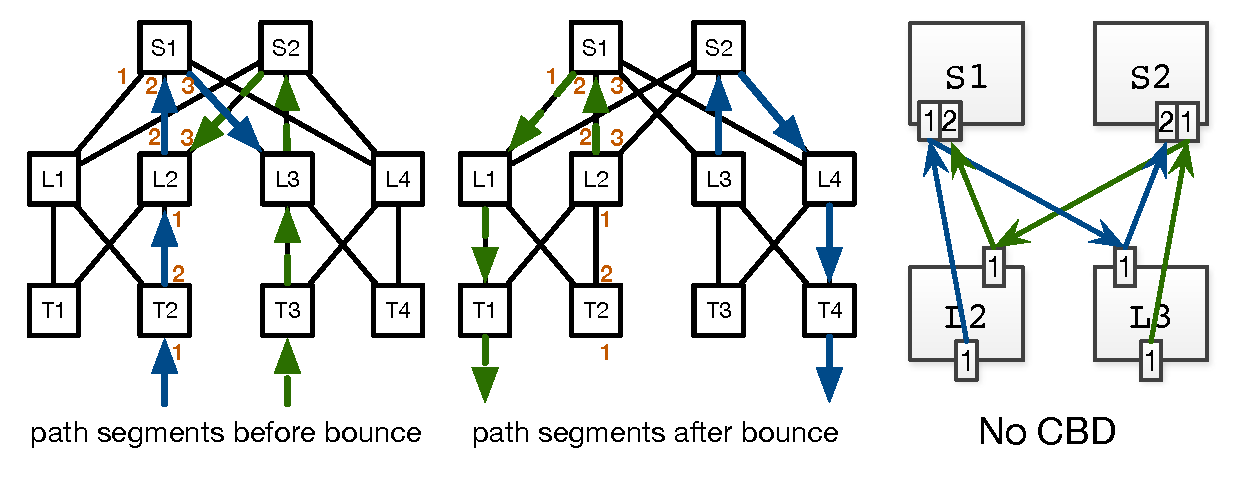
\includegraphics[width=0.5\textwidth] {figs/cbd_b}
	}
	
	\caption{Micropath based priority transition can eliminate CBD.}\label{fig:priority_transition}
\end{figure}



Figure~\ref{fig:priority_transition}(a) shows a simple Clos topology. In addition to shortest path routing, the operators also
require the ``1-bounce'' paths to be lossless to mitigate the impact of failed links/switches. 
Unfortunately, multiple ``1-bounce'' paths together may form CBD and cause deadlock (Figure~\ref{fig:priority_transition}(a))~\cite{mellanox}.

However, if we divide the paths into two segments, {\em before-bounce} and {\em after-bounce}, and assign them to
different priority queues, there is no more CBD (Figure~\ref{fig:priority_transition}(b)). 
The insight we get from this example is that if the switch can detect that a packet may cause CBD in next hops,
it can change the packet's priority to avoid CBD, thus avoiding deadlock. 

This is different from the prior solutions, which either assign a fixed priority based on pre-compute paths (cannot 
react to dynamic routing), or change the priority every hop (requires too many priority queues). Instead, we chop 
the paths into a few segments, which we call {\em micropaths},
and change packet's priority only at a few transition point. It has the advantages from both types of prior work,
{\em i.e.,} it requires a small number of priroties, and allows the switch to react to each packet's path.

The key enabler of our approach is the topology and the set {\em lossless routes} specified by the operators
as the input. By properly dividing lossless routes into multiple subspaces of micropaths, we can
ensure that CBD is eliminated {\em within} each subspace. Section~\ref{sec:greedy} shows a way to achieve this.

Inevitably, we will need {\em multiple} switch lossless queues to support one lossless application class.
Specifically, we divide the buffer of network nodes into $k$ partitions, and let the $j$-$th$ partition associated 
with priority queue $j$. If a packet is classified into priority queue $j$, it will be buffered in the $j$-$th$ buffer 
partition and can generate PFC of priority $j$. 

In this section, we focus on supporting {\em just one} lossless application class. In Section~\ref{sec:specific}, we will revisit 
this issue and show how we may support multiple application classes more efficiently.

\subsection{Idea 2: Tag for Ordered Micropath Subspaces}\label{sec:tag_order}

\begin{figure}[t]
	%\vspace{-0.1in}
	\centering
	
	\subfloat[short for lof][CBD among subspaces.] {
		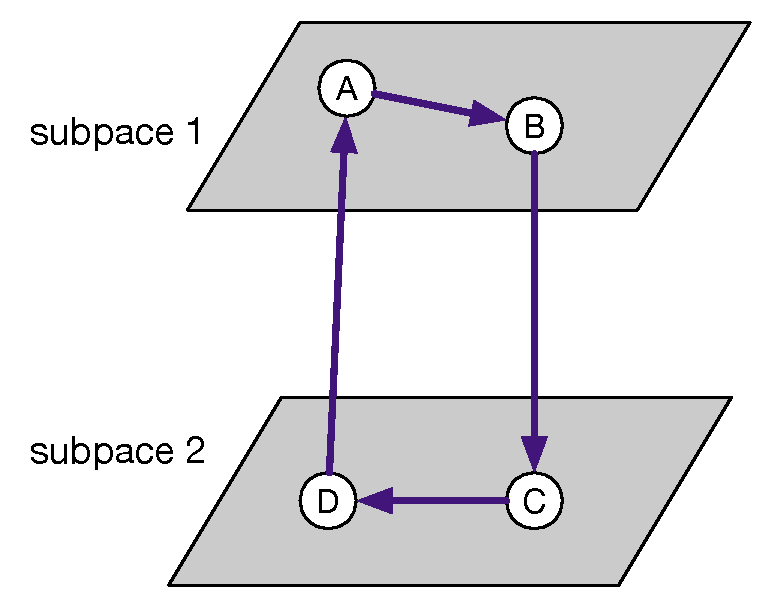
\includegraphics[width=0.24\textwidth] {figs/subspace_a}
	}
	\subfloat[short for lof][Ordered subspaces.]{
		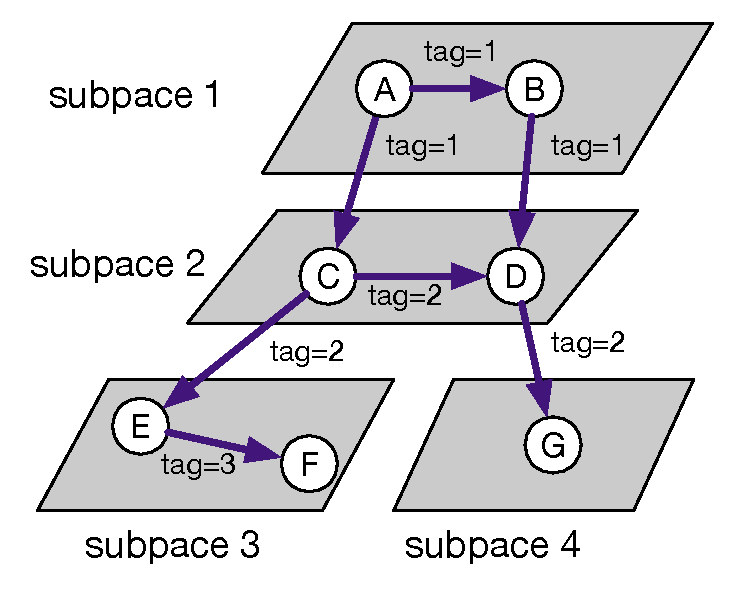
\includegraphics[width=0.26\textwidth] {figs/subspace_b}
	}
	
	\caption{Ordered subspaces ensure deadlock-free priority transition.}\label{fig:subspace}
\end{figure}


Even though proper micropath partition ensures no CBD {\em within} each priority, packets can still cause CBD
{\em across} priorities, as shown in Figure~\ref{fig:subspace}(a). Switch must know the past path of each packet in order to decide the priority that avoids CBD.

As shown in Figure~\ref{fig:subspace}(b), We enforce the order of transitioning among micropath subspaces and tag only based on current subspace.
With this, the packets do not need to record the whole history of past micropaths in headers. A fixed length 
header field (most commonly, DSCP) is sufficient to carry the tag. The tag values are one-one mapped to the micropath subspaces,
which one-one maps to priority queues on each switch. 

With this idea, we design the tag system in Tagger. In this system, each switch enqueues each packet into priority queue based
on its tag, and changes the tag if the switch decides to change the packet's priority at the next hop.
We can prove that the network is deadlock-free if the tag system, which defines micropath subspaces and transition, 
satisfies the two requirements below:

\begin{enumerate}

	\item A packet's tag is unchanged or changed at each hop of its path. When the tag is changed, it must be changed monotonically 
	along any packet's path (e.g., always increasing).

	\item For any given tag, all micropaths within the corresponding micropath subspace do not form cyclic buffer dependency.

\end{enumerate}

\para{Proof of deadlock-free}


\textbf{Claim:} Any tag system that satisfies the above two requirements is deadlock-free regardless of the 
packet scheduling algorithms on any swithes.

\textbf{Proof:} We prove by contradiction that no legal buffer state can be in deadlocked buffer state.

\fixme{Need to rewrite the below symbols.}

Assuming there exists a legal buffer state $BS_N(t)$ which is also a deadlocked buffer state. If no new packets are injected into 
the network since time $t$, according to Equation~(\ref{eqn:deadlockstatedef}), $BS_N(t)$ will converge into a fixed non-empty 
buffer state $BS_N(t_0)$ at some finite time $t_0>t$. 


\textbf{Case 1:} All the VEQs in $BS_N(t_0)$ is empty. As $BS_N(t_0) \neq BS^0_N$, $BS_N(t_0)$ has at least one non-empty VIQ. 
As $BS_N(t)$ is a legal buffer state, accroding to Equation~(\ref{eqn:legalstatecon}), there are finite number of packets queued 
in non-empty VIQs of $BS_N(t_0)$. Then according to Equations~(\ref{eqn:schecon1}), (\ref{eqn:nodupschedule}) and (\ref{eqn:fwdcon}), 
any unscheduled packet remaining in any VIQ will be forwarded to some VEQ within finite time at some finite time $t_2>t_0$. 
This means that $BS_N(t_0)$ will transition to some other buffer state, which violates the fact that 
$\forall t_1>t_0, BS_N(t_1)\equiv BS_N(t_0)$.

\textbf{Case 2:} There exist some non-empty VEQs (at least one) in $BS_N(t_0)$. Let $q_{out}^{i,m}$ be the queue of highest priority 
class among all the non-empty VEQ queues ($m\leq k$). Packets in $q_{out}^{i,m}$ will not be paused 
by PFC PAUSE messages as packets can only be paused by packets of higher priority class. According to Equations~(\ref{eqn:schecon2}) 
and (\ref{eqn:transcon}), packets in $q_{out}^{i,m}$ will be transmitted to next hop within finite time. This means that $BS_N(t_0)$ 
will transition to some other buffer state at some finite time $t_2>t_0$, which violates the fact that 
$\forall t_1>t_0, BS_N(t_1)\equiv BS_N(t_0)$.

Based on the above discussion, the assumption we made will cause contradiction in both cases. Hence $BS_N(t)$ is not a deadlocked 
buffer state. So any tag-based solution that satisfies the above two requirements is deadlock-free regardless of the packet 
scheduling algorithms.

In short, this idea guarantees that the deadlock is eliminated while avoiding modifying packet headers.


\subsection{Idea 3: Minimizing the Number of Micropath Subspaces} 
The number of micropath subspaces (or tags) is essentially the number of lossless queues required on each switch.
We must reduce it to below the switch hardware limit. In this section, we focus on hte number of lossless queues for 
just ONE application class. We first formalize this optimization problem.

\para{Notations.} Let $A_i$ represent a unique ingress port in the network, {\em i.e.,} switch $A$'s $i^th$ ingress port.
With a tagging system, each port may receive packets with different tags.
$(A_i, x)$ is a port-tag pair: the case where $A_i$ gets a packet with tag $x$.
$V$ is the set of all possible port-tag pairs. 

Between these port-tag pairs, there exists an edge $(A_i, x)\rightarrow(B_j, y)$ {\em iff.} switch $A$ and $B$ are 
connected, AND switch $A$ may change a packet's tag from $x$ to $y$ before sending to $B$ (the case $i=j$ also counts).
It is essentially a buffer dependency -- whether $A_i$ can dequeue packets depending on whether $B_j$ has paused upstream.
$E$ is the set of all such edges. We call $G(V, E)$ the tagged graph.

The tags define a partition of the tagged graph, $\{G_k\}$, where $G_k = \{(A_i, k) | \forall A, i\}$.
Each $G_k$ is a {\em micropath subspace}. We assign a separate lossless priority to each $G_k$.

A brute-force solution is to monotonically change the tag (thus, the priority) every hop.
It is easy to verify that CBD is eliminated. However, it requires too many lossless queues in a large network.
We want to minize the number of lossless queues by leveraging the routing information.

%\textbf{Input:} the lossless graph $G(V, E)$, defined by Table~\ref{tab:symbols}
\para{Algorithm goal:} find a tagging system that minimizes $|\{G_k\}|$, {\em s.t.,}
\begin{enumerate}
\item Any $G_i$ does NOT have a cycle, because a cycle means the possiblity of CBD.
\item There is no lossless route going from $G_i$ to $G_j$ if $i \l j$ (monotonically non-increasing transision).
\end{enumerate}

The two requirements correspond to the requirements stated in Section~\ref{sec:tag_order}.

\begin{table}
\small
\centering
\caption{Notations in the formalized problem description.}
\label{tab:symbols}
\begin{tabular}{|c|c|}
\hline
Symbol & Description \\ \hline
$A_i$ & Switch $A$'s $i^{th}$ ingress port  \\ \hline
$(A_i, x)$ & A port-tag pair \\ \hline
$(A_i, x)\rightarrow(B_j, y)$ & A hop \\ \hline
$V$ & All port-tag pairs in lossless paths  \\ \hline
$E$ & All tagged hops \\ \hline
$G(V, E)$ & Tagged graph \\ \hline
\end{tabular}
\end{table}

\if 0
\para{Start point: brute-force tag system.} A strawman solution is to monotonically change the tag (thus, the priority) every hop.
This is a degenerate version of our micropath-based solution.
Initially, the tag of all packets is set to $tag_0$. The tag value decreases by one every hop. 
Let $tag_i$ be the tag value of a packet at its $i$-$th$ hop ($i \geq 0$). At every hop, 
set the tag (priority) of any incoming packet $p$ to be $tag_0 - tag_i$. 
It is easy to verify that this satisfies the two requirements above: the tag changes monotonically, and there is no CBD
within each micropath subspace.
However, the drawback of such tagging is that it requires too many lossless queues. 
\fi

%\subsubsection{Proof of Deadlock-free Property}\label{subsec:proof}
%In this part, we are going to prove that our TTL-based solution is deadlock-free regardless of the packet scheduling algorithms.

%In our proof, we use $p_{size}$, $p_{ttl}$ and $p_{dst}$ to denote the size, the TTL value and the destination of a packet $p$, respectively. Any ingress queue $q_{in}^{i,j}$ and any egress queue $q_{out}^{i,j}$ are viewed as packet sets. According to the switch model, we have $q_{in}^{i}=\cup_{j=1}^{k}q_{in}^{i,j}$, and $q_{out}^{i}=\cup_{j=1}^{k}q_{out}^{i,j}$.

%We use $|q_{in}^{i,j}|$ and $|q_{out}^{i,j}|$ to denote the queue lengths of $q_{in}^{i,j}$ and $q_{out}^{i,j}$, where $|q_{in}^{i,j}|=\sum_{p\in q_{in}^{i,j}}p_{size}$, and $|q_{out}^{i,j}|=\sum_{p\in q_{out}^{i,j}}p_{size}$.


\para{Greedy algorithm.} We design Algorithm~\ref{alg:greedy} for the above goal.
It works by greedily combining as many micropaths as possible into each micropath subspaces under CBD-free constraint.
To ensure the monotonic property, we use the brute-force solution as the starting point. We start from combing the port-tags 
with largest tag to smallest tag in the brute-force solution,
the monotonic property will still hold after combination. 


\begin{algorithm}
    \KwIn{The brute-force tagged graph $G(V, E)$}
	\KwOut{A partition of $G$}
	$G_x \gets Set()$ array $[0..maxTag]$\; 
	$i \gets 0$\;
	\For{$t \gets maxTag$ \textbf{downto} $minTag$} {
		\For{each $v$ in $V$ whose tag is $t$} {
			$G_i' \gets G_i \cup \{v\}$ \;
			\uIf{MergeNodesByPorts$(G_i')$ is acyclic} {
				$G_i \gets G_i'$ \; 
			}
			\Else{
				$G_{i+1} \gets G_{i+1} \cup \{v\}$\;
			}
			$V \gets V \backslash \{v\}$ \;
		}
		\uIf{$G_{i+1}$ is not empty} {
			$i \gets i+1$\;
		}
	}
	\Return{$\{G_0, G_1, ...\}$}\;
    \caption{Greedily minimizing the number of micropath subspaces by merging brute-force tags.}
	\label{alg:greedy}
\end{algorithm}

In the end, we assign a new tag (different from the brute-force tag) for each micropath subspace, and generate switch configurations
based on the new tags. The worst case scenario is as bad as using the brute-force tags, which require
as many priority queues as the longest route in lossless routes. However,
in Section~\ref{sec:eval}, we show that this algorithm works reasonably well for generic topology, like Jellyfish. 

This greedy algorithm may not always return the optimal solution. For example, the result it gives for Clos network is not 
optimal! In Section~\ref{sec:specific}, we show that for structured topology, smarter tagging system can achieve optimal results.

%\begin{figure}[t]
%	%\vspace{-0.1in}
%	\centering
%	
%	\subfloat[short for lof][Topology and routes.] {
%		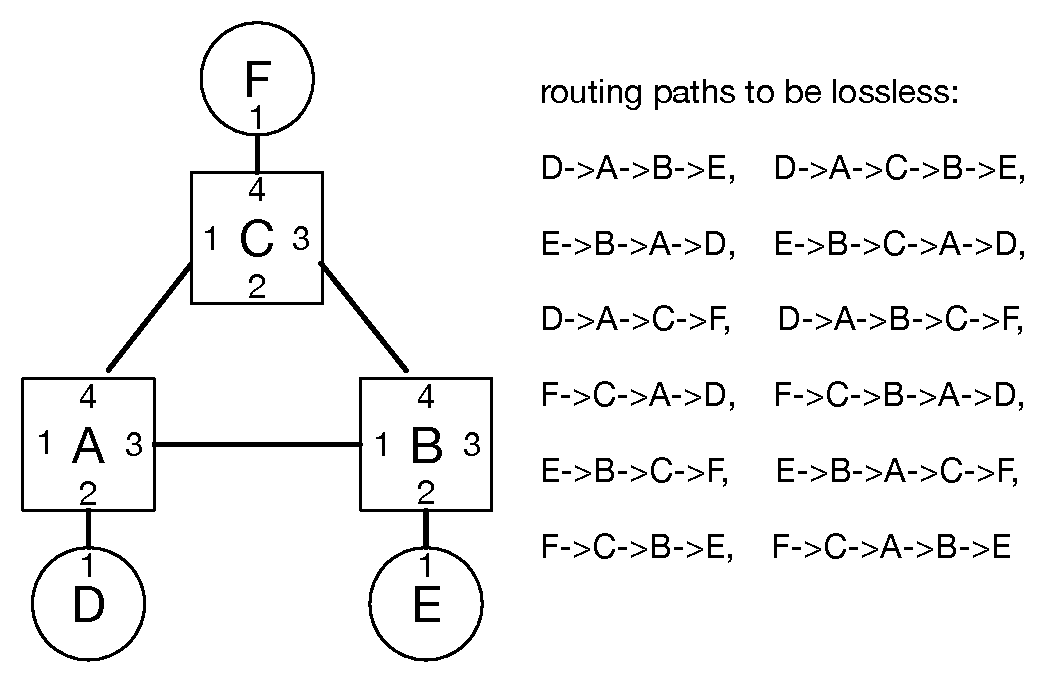
\includegraphics[width=0.45\textwidth] {figs/alo_walkthrough_a}
%	}
%
%	\subfloat[short for lof][Tagged graph.]{
%		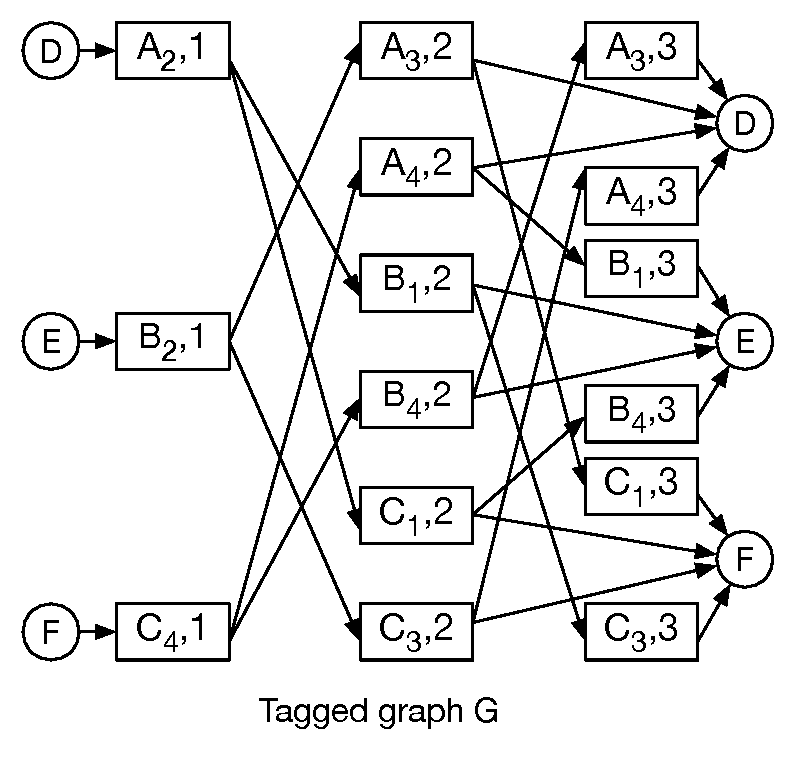
\includegraphics[width=0.45\textwidth] {figs/alo_walkthrough_b}
%	}
%	
%		\subfloat[short for lof][Partitions of tagged graph.]{
%		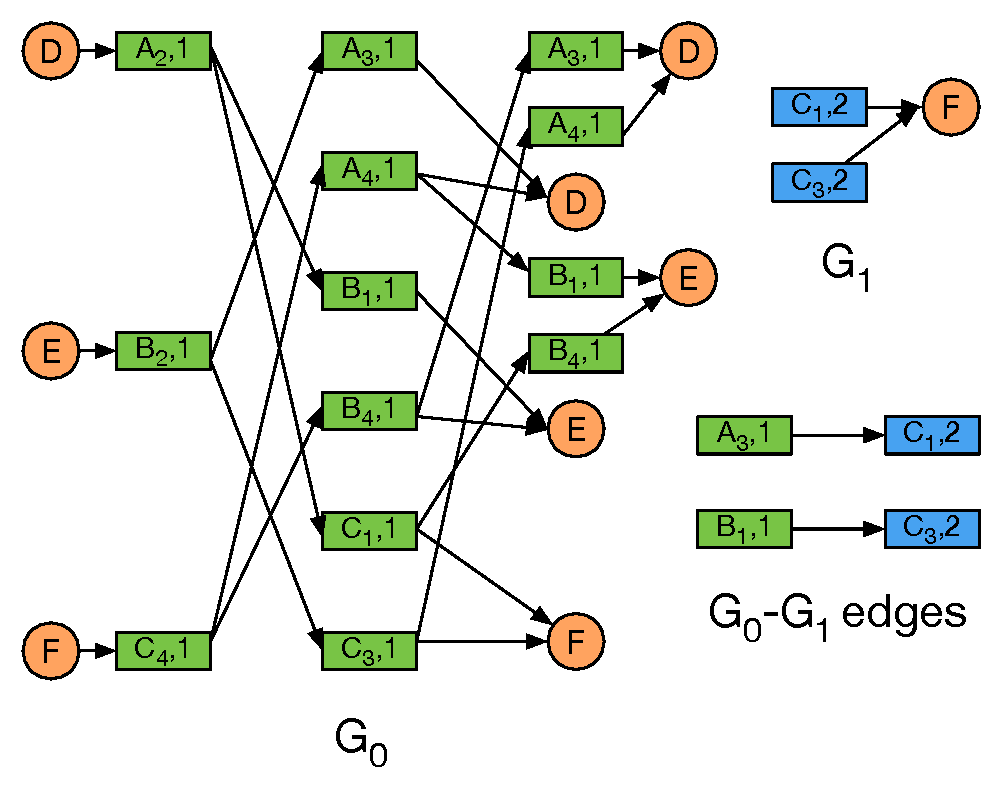
\includegraphics[width=0.45\textwidth] {figs/alo_walkthrough_c}
%	}
%	\caption{Walk-through example for the  algorithm.}\label{fig:subspace}
%\end{figure}
